% Adding a coloured vertical edge to the pages in the chapter
\ClearShipoutPicture
\AddToShipoutPicture{%
  \AtPageLowerLeft{%
    \checkoddpage
    \ifoddpage
      \begin{tikzpicture}[remember picture,overlay] % Odd page → right edge
        \draw[line width=80pt, colour_chapter7] 
             (\paperwidth,0) -- (\paperwidth,\paperheight);
      \end{tikzpicture}%
    \else
      \begin{tikzpicture}[remember picture,overlay] % Even page → left edge
        \draw[line width=80pt, colour_chapter7] 
             (0,0) -- (0,\paperheight);
      \end{tikzpicture}%
    \fi
  }%
}

%%%%%%%%%%%%%%%%%%%%%%%%%%%%%%%%%%%%%%%%%%%%%%%%%%%%%%%%%%%%%
\chapter{Towards predictions over a continuous global domain: 
global implementation of regionally-trained models}
\label{regional_to_global_training}
\graphicspath{{chapter_07/figures}{chapter_07/tables}}

\definecolor{colourTraining}{HTML}{800080}
\definecolor{colourTest}{HTML}{00B0F0}
%%%%%%%%%%%%%%%%%%%%%%%%%%%%%%%%%%%%%%%%%%%%%%%%%%%%%%%%%%%%%

\underline{\textbf{Authors' contribution for this chapter:}} Fatima M. Pillosu designed the study, with advice from Hannah Cloke and Christel Prudhomme, obtained the datasets, carried out the analysis, and led the writing of the manuscript. All authors assisted with writing the manuscript. Overall, 90\% of the writing was undertaken by Fatima M. Pillosu.

\vspace{\baselineskip}

\section*{PREFACE}
\addcontentsline{toc}{section}{PREFACE}



\clearpage

\section*{ABSTRACT}
\addcontentsline{toc}{section}{ABSTRACT}

\clearpage



%%%%%%%%%%%%%%%%%%%%%%
\section{Introduction}
\label{regional_to_global_training_introduction}

The aspiration to develop predictions of areas at risk of flash floods over a continuous global domain confronts a fundamental paradox that extends beyond technical challenges to encompass critical questions of equity in disaster risk reduction and preparedness. Flash floods represent one of the most devastating natural hazards globally, affecting populations in the Global North and Global South equally. However, the observational infrastructure necessary for developing predictive models that can help the population prepare and mitigate the risk against flash floods remains concentrated in a small subset of wealthy nations. This disparity violates the principle that all populations, regardless of their location or economic status, should have access to life-saving flood warnings — a goal central to the UN's 'Early Warnings for All' initiative. Moreover, as flash floods typically occur in poorly gauged catchments, this further reduces the number of observations available for model development and post-hoc event analysis even in data-rich regions in the Global North, thereby hindering our understanding of flash flood generation mechanisms. This inequitable distribution of observational capacity to assess flash flood occurrence creates an urgent need for innovative approaches that can transcend the limitations of traditional catchment-specific modelling paradigms to develop predictive models over a continuous domain able to truly cover all populations around the globe.

The emergence of data-driven approaches in large-sample hydrology has demonstrated remarkable success in learning complex relationships between hydro-meteorological variables and flood occurrence. Many data-driven applications are also now applied to predict areas at risk of flash floods or river discharge in flashy catchments. However, such applications remain primarily at the catchment level due to the aforementioned severe paucity of observations suitable for predicting flash flood events. There exist only a few examples of prediction systems at a larger scale (e.g., national).

Recent advances in transfer learning and domain adaptation offer a transformative approach to this challenge. Rather than requiring comprehensive local observations for model training, one could train a data-driven model to learn generalisable hydro-meteorological relationships from data-rich regions and subsequently deploy the model to create predictions over a continuous global domain, provided that hydro-meteorological variables from global NWP models are used. The key insight underlying this approach is that whilst specific catchment characteristics may vary globally, the fundamental physical processes governing flash flood generation — the interaction between intense precipitation, antecedent soil moisture, topography, and land surface characteristics — exhibit sufficient commonality to enable knowledge transfer across different regions.

The development of such transferable models faces a critical trade-off between spatial coverage and data density. Models trained on high-density observations from limited geographical regions may capture local flash flood dynamics with high fidelity, but may fail to generalise to regions with different climatic regimes, topographies, or land use patterns. Conversely, models trained on sparse global datasets may achieve broader applicability but at the cost of reduced accuracy in the overall identification of areas at risk of flash floods. 

This chapter addresses Research Question 3 of this thesis by systematically investigating how the coverage-density trade-off influences training strategies for developing predictions of areas at risk of flash floods over a continuous global domain. Building upon the data-driven models developed in Chapter \ref{data_driven_flash_floods_short_medium_range}, we explore three distinct approaches to training data selection through sensitivity analysis over the CONUS domain. Approach 1 employs random spatial sampling that maintains geographical coverage across the full CONUS domain whilst reducing overall observation density. This approach simulates conditions analogous to global model training using sparse impact reports from databases such as EM-DAT. The model is exposed to the entire global domain with impact reports distributed across the globe, but at an extremely low observational density—tens of times lower than the already sparse 0.27\% coverage of the Storm Event Database. Approach 2 utilises regionally-constrained training with global visibility. The model trains on flash flood observations from only a subset of the spatial domain whilst maintaining exposure to the full domain during training. This approach simulates conditions where the model learns from the full global domain but receives impact reports only from data-rich regions such as the USA and Europe. Consequently, the model learns that certain regions appear to have no flash flood occurrences. This approach investigates whether such training affects the model's ability to predict areas at risk of flash floods in regions where no events have been observed. Approach 3 implements domain-exclusion training, where the model trains exclusively on a geographically restricted subset without exposure to regions lacking observations. This approach simulates conditions where the model only encounters geographical domains with higher observational density, completely excluding areas with no observations or poor coverage. This method examines the implications for flash flood risk predictions in the excluded regions and tests the model's capacity for spatial extrapolation to entirely unseen geographical areas.

% Complete the ending for the introduction.


%%%%%%%%%%%%%%%%%%%%%%%%%%
\section{Methods and Data}
\label{regional_to_global_training_methods_data}

\subsection{Training approaches}
The methodological framework examines three distinct training strategies to determine the optimal approach for developing flash flood predictions across a continuous global domain, considering heterogeneous data availability. 

\begin{figure}[htbp]
\centering
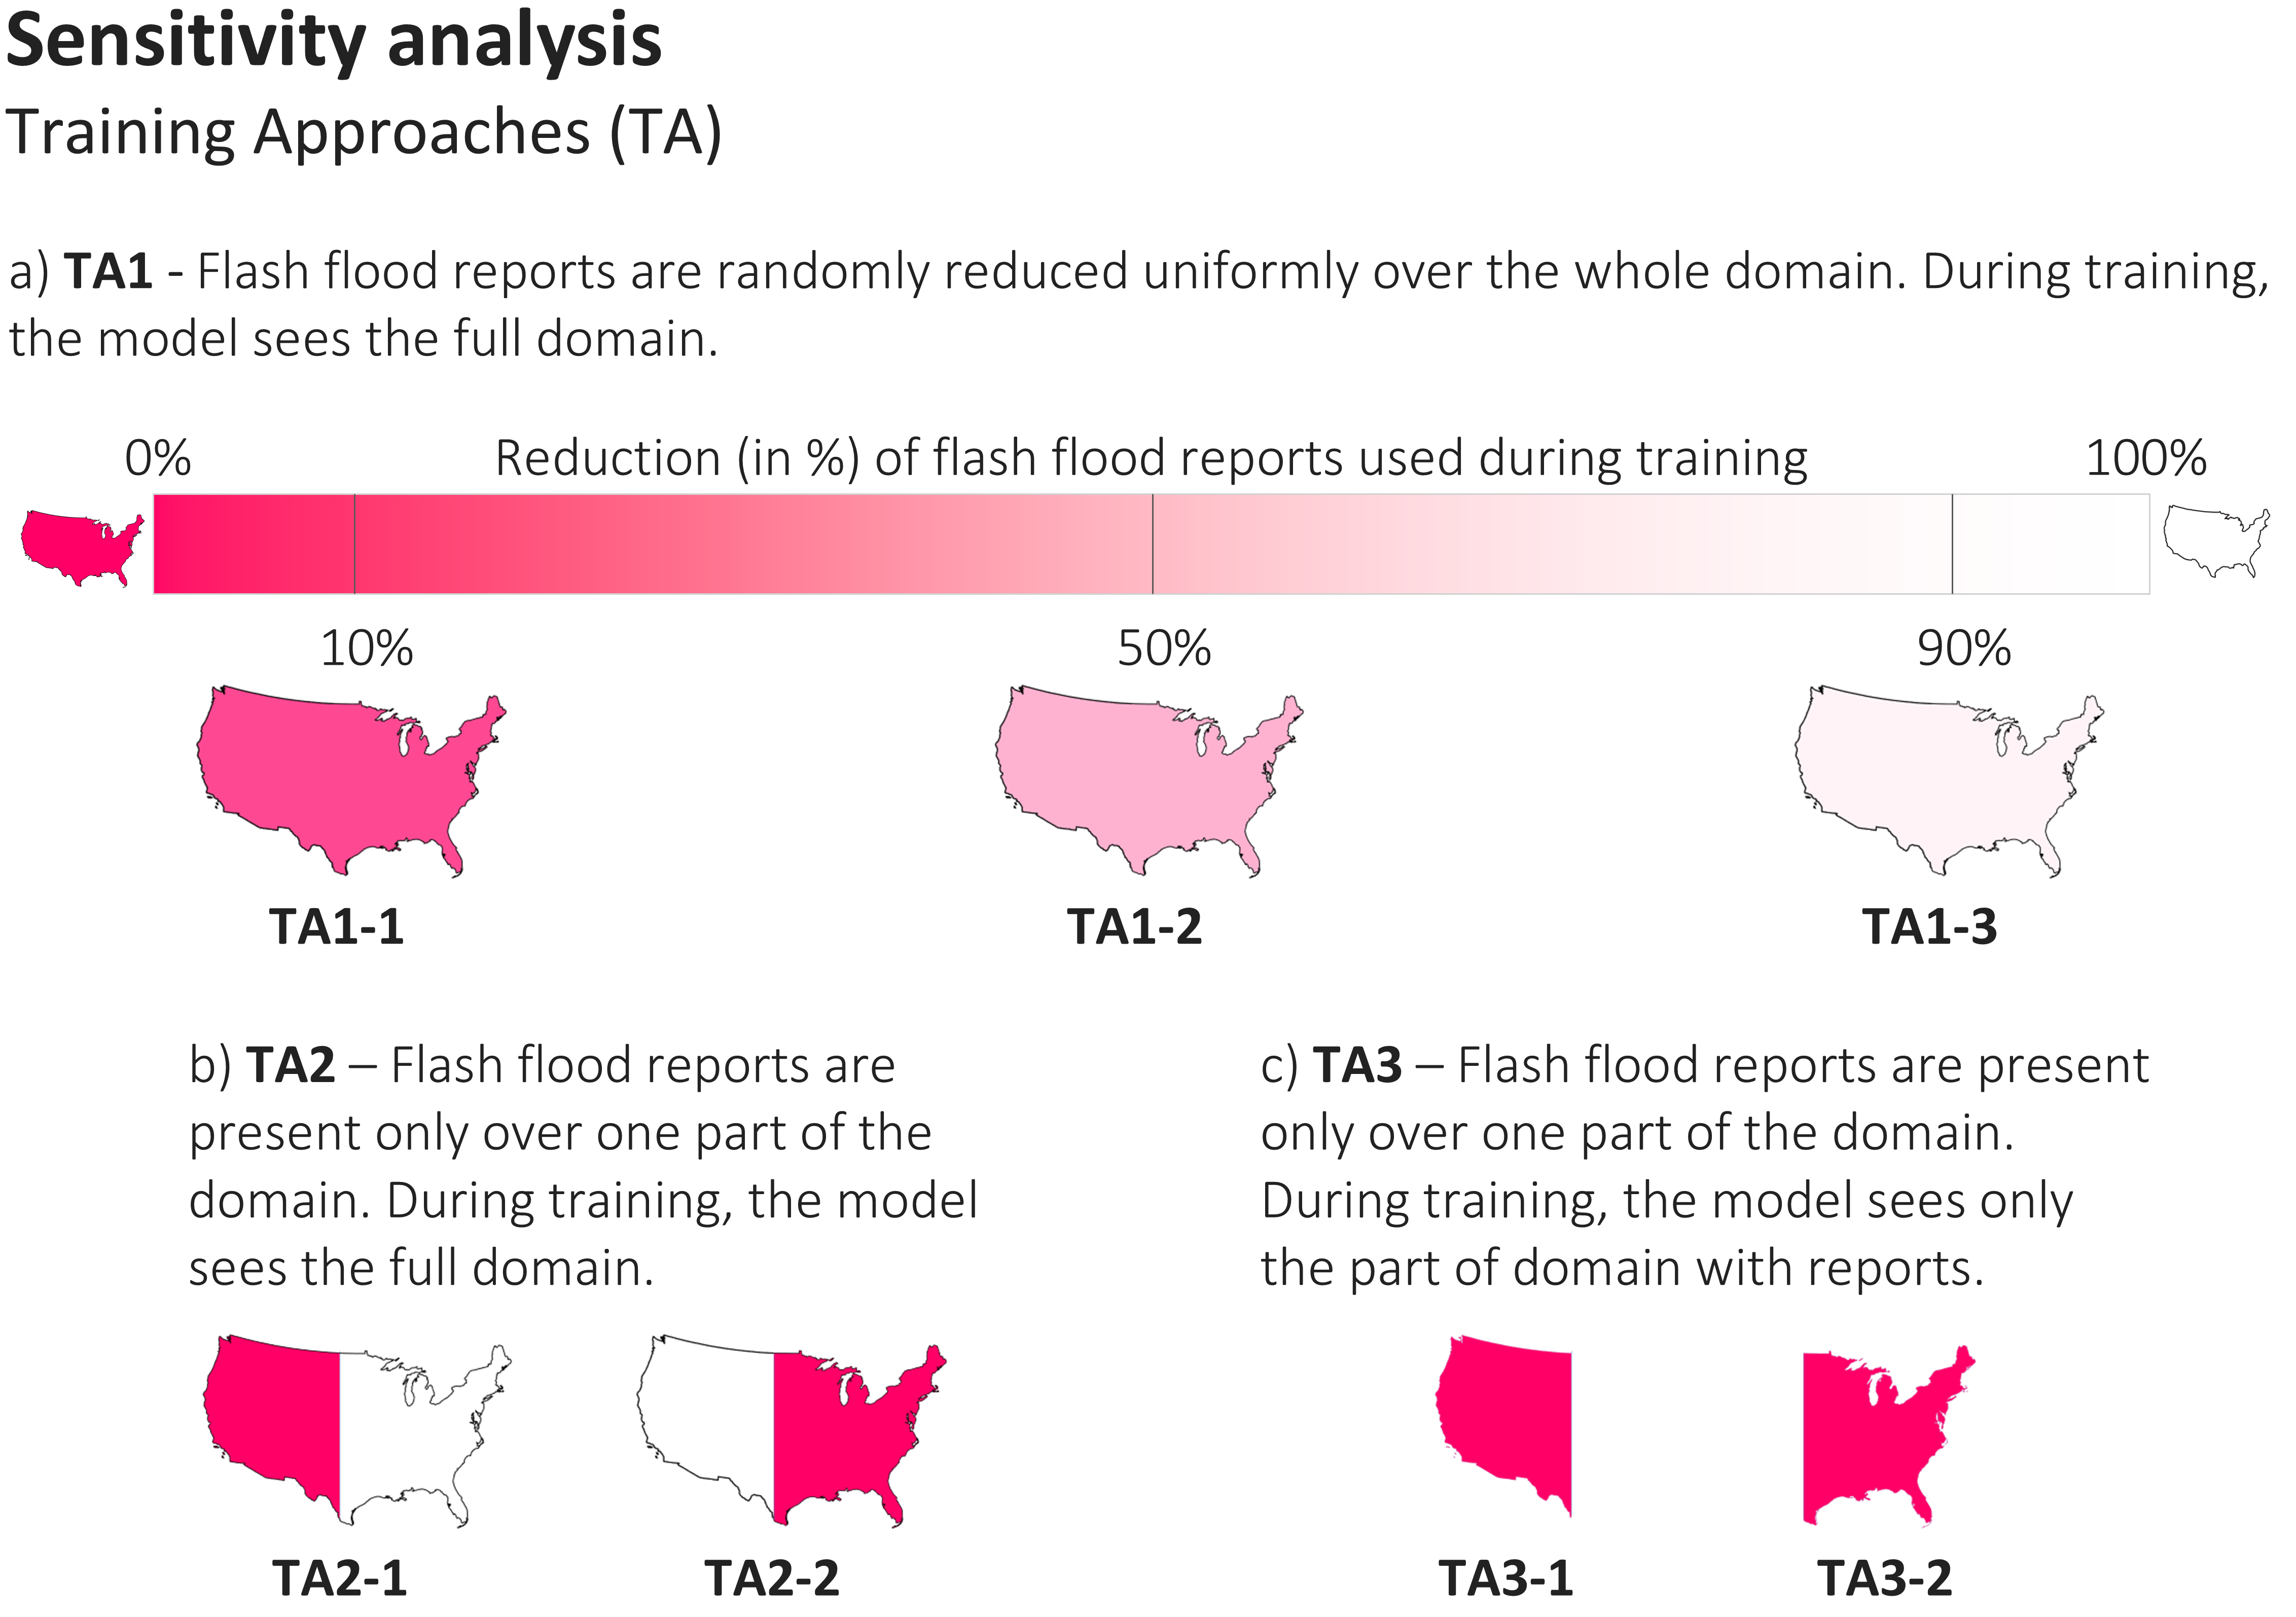
\includegraphics[width=\textwidth]{training_approaches.png}
\caption{\textbf{Training approaches adopted in the sensitivity analysis.} Panel (a) describes Training Approach 1 (TA1) - where the flash flood reports are randomly reduced uniformly over the whole domain by 10\% (TA1-1), 50\% (TA1-2), and 90\% (TA1-3), and during training, the model sees the full domain. Panel (b) describes Training Approach 2 (TA2) - where the flash flood reports are present only over one part of the domain (TA2-1 for reports in the west and TA2-2 in the East), but during training, the model still sees the full domain. Panel (c) describes Training Approach 3 (TA3) - where the flash flood reports are present only over one part of the domain (TA3-1 for reports in the west and TA3-2 in the East), and during training, the model sees only the part of the domain with reports.}
\label{fig:training_approaches}
\end{figure}

This \marginpara{Training approach 1 (TA1)} approach tests whether training over the full CONUS domain remains effective when flash flood observations are systematically reduced. Flash flood reports from the Storm Event Database were randomly sampled at three levels: 90\%, 50\%, and 10\% of the original dataset. The sampling was applied uniformly across the entire domain, maintaining the spatial distribution whilst reducing observation density. This approach simulates the scenario of training a global model with sparse but spatially distributed observations.

The \marginpara{Training approach 2 (TA2)} second approach maintains training over the full CONUS domain but restricts flash flood observations to specific regions. Unlike Approach 2, the model receives hydro-meteorological data from the entire domain during training but only has access to flash flood labels in the selected region. The non-selected regions contribute only negative samples (non-flood events) to the training dataset. This configuration simulates the realistic scenario of developing a global model where flash flood reports are available only from certain countries or regions, whilst meteorological data has global coverage.

The \marginpara{Training approach 3 (TA3)} third approach examines whether models trained on high-quality observations from limited geographical regions can effectively predict flash floods in areas where they have never observed any events. The CONUS domain was divided into four regions: East (east of 98°W), West (west of 98°W), North (north of 37°N), and South (south of 37°N). For each configuration, the model was trained using flash flood observations from only one region, with the remaining regions containing no observations during training. The trained model was then applied to predict flash floods across the entire CONUS domain. This approach directly addresses the scenario where certain parts of the world have excellent observational infrastructure, whilst others have none.

The spatial divisions for Approaches 2 (Figure \ref{fig:training_approaches}b) and 3 Figure \ref{fig:training_approaches}c were selected to create regions with varying flash flood characteristics. Two main regions were selected. The eastern region (east of the longitude 100°W) encompasses mostly flat regions (except for the Appalachian Mountains), is highly populated, and is frequently affected by convective storms and hurricanes. The western region (west of the longitude 100°W) encompasses mostly mountainous regions (except for the Central-North Pacific coast), is less populated, and is more frequently affected by large-scale systems bringing large amounts of rainfall due to orographic enhancement.

\subsection{Training data configuration}
For all training approaches, the baseline configuration consists of the full Storm Event Database over the CONUS as presented in Chapter \ref{datasets}. The hydro-meteorological features - including ERA5-ecPoint rainfall, ERA5 antecedent soil moisture, vegetation coverage and topography steepness - also remain consistent with those presented in Chapter \ref{datasets} and already used in Chapter \ref{data_driven_flash_floods_short_medium_range}. The training period remains between 2001 and 2020, as well as the verification period from 2021 to 2024.

\subsection{Model configuration}
The analysis employs the XGBoost model developed in Chapter \ref{data_driven_flash_floods_short_medium_range}. The model's hyperparameters remain consistent with those optimised in Chapter \ref{data_driven_flash_floods_short_medium_range} to ensure that performance differences arise solely from training data modifications (exemplified by TA1-3) rather than model architecture changes. 
 
\subsection{Performance evaluation}

Model performance will first be evaluated by determining how the \textit{distribution of predicted probabilities} changes between the three considered training approaches. Thus, violin plots will be built with the predicted probabilities obtained from training the XGBoost model with TA1-3. As a second model performance assessment, the \textit{flash flood detection capability} for the three different training approaches will be assessed. This will be achieved by computing the different number of grid cells indicating a yes-event between the predictions obtained from one of the TAs and the model trained with the full observational dataset (as computed in Chapter \ref{data_driven_flash_floods_short_medium_range}).

Following the assessments mentioned above, objective verification for the three TAs will be carried out over the full CONUS domain, and the results will be compared to those obtained in Chapter \ref{data_driven_flash_floods_short_medium_range} using the complete training dataset. Such a comparison will determine any potential degradation in predictive performance for any of the three TAs. Hence, the same verification scores adopted in Chapter \ref{data_driven_flash_floods_short_medium_range} will also be considered in this chapter, i.e. ROC curves, precision-recall curves, and reliability diagrams as breakdown scores. Area under the ROC (AUC-ROC) and under the precision-recall curves (AUC-PR), together with the frequency bias (FB) will also be considered as overall scores for discrimination ability (AUC-ROC and AUC-PR) and reliability (FB).
 
The verification assessments will conclude with a case-study-based analysis. This type of \textit{subjective} analysis is preferred to analyse the performance of the global predictions because global impact datasets, such as EM-DAT and DesInventar, do not contain enough observations to compute robust statistics from objective verification (as done over the CONUS). For the US, predictions of areas at risk of flash floods obtained from the three TAs will be presented again for Storm Ida (for more details on the specific event, refer to Chapter \ref{datasets}). Moreover, this US-focused case study will be complemented in this chapter by case studies from other parts of the world: the flash floods in Valencia, Spain, in 2024 and in China, in 2021. Both represent extremely severe flash flood events that caused high death tolls and considerable economic losses. However, the first will represent a very localised flash flood event, generated by a small-scale convective system. In contrast, the second will represent a widespread flash flood event, generated by a large-scale convective system. These two events were chosen due to their inherent differences in predictability.


%%%%%%%%%%%%%%%%%
\section{Results}
\label{regional_to_global_training_results}

The \marginpara{Objective verification: overall scores (AUC-ROC, AUC-PR, FB)} area under the ROC curve (AUC-ROC, Figure \ref{fig:verif_overall_scores}a) and the area under the precision-recall curve (AUC-PR, Figure \ref{fig:verif_overall_scores}b) show that TA1 and TA3 achieve very close and close discrimination ability to those achieved by the model trained with the complete training dataset (dash lines). TA2 is the approach that reduces the most the discrimination ability. In particular, TA2-1 reduces both AUC-ROC and AUC-PR by \sim20\% (from 0.8 to 0.57 and from 0.025 to 0.0024). For TA1, the frequency bias (FB) diminishes with increasing reductions of flash flood reports in the training dataset, and it reaches values close to 0 - \sim0.2 - for TA1-3. The datasets in TA2 and TA3 show opposite behaviours. TA2-1 and TA3-1 (which consider reports only over the West part of the CONUS) show poorer FBs with an overall tendency to underestimate the occurrence of flash floods. In particular, TA2-1 shows an extremely low FB = 0.0022. TA2-2 and TA3-2 (which consider reports only over the East part of the CONUS) show the closest values to those obtained for the model trained with the complete training dataset, even though with a slight tendency to underestimate the frequency of flash floods.

\begin{figure}[htbp]
\centering
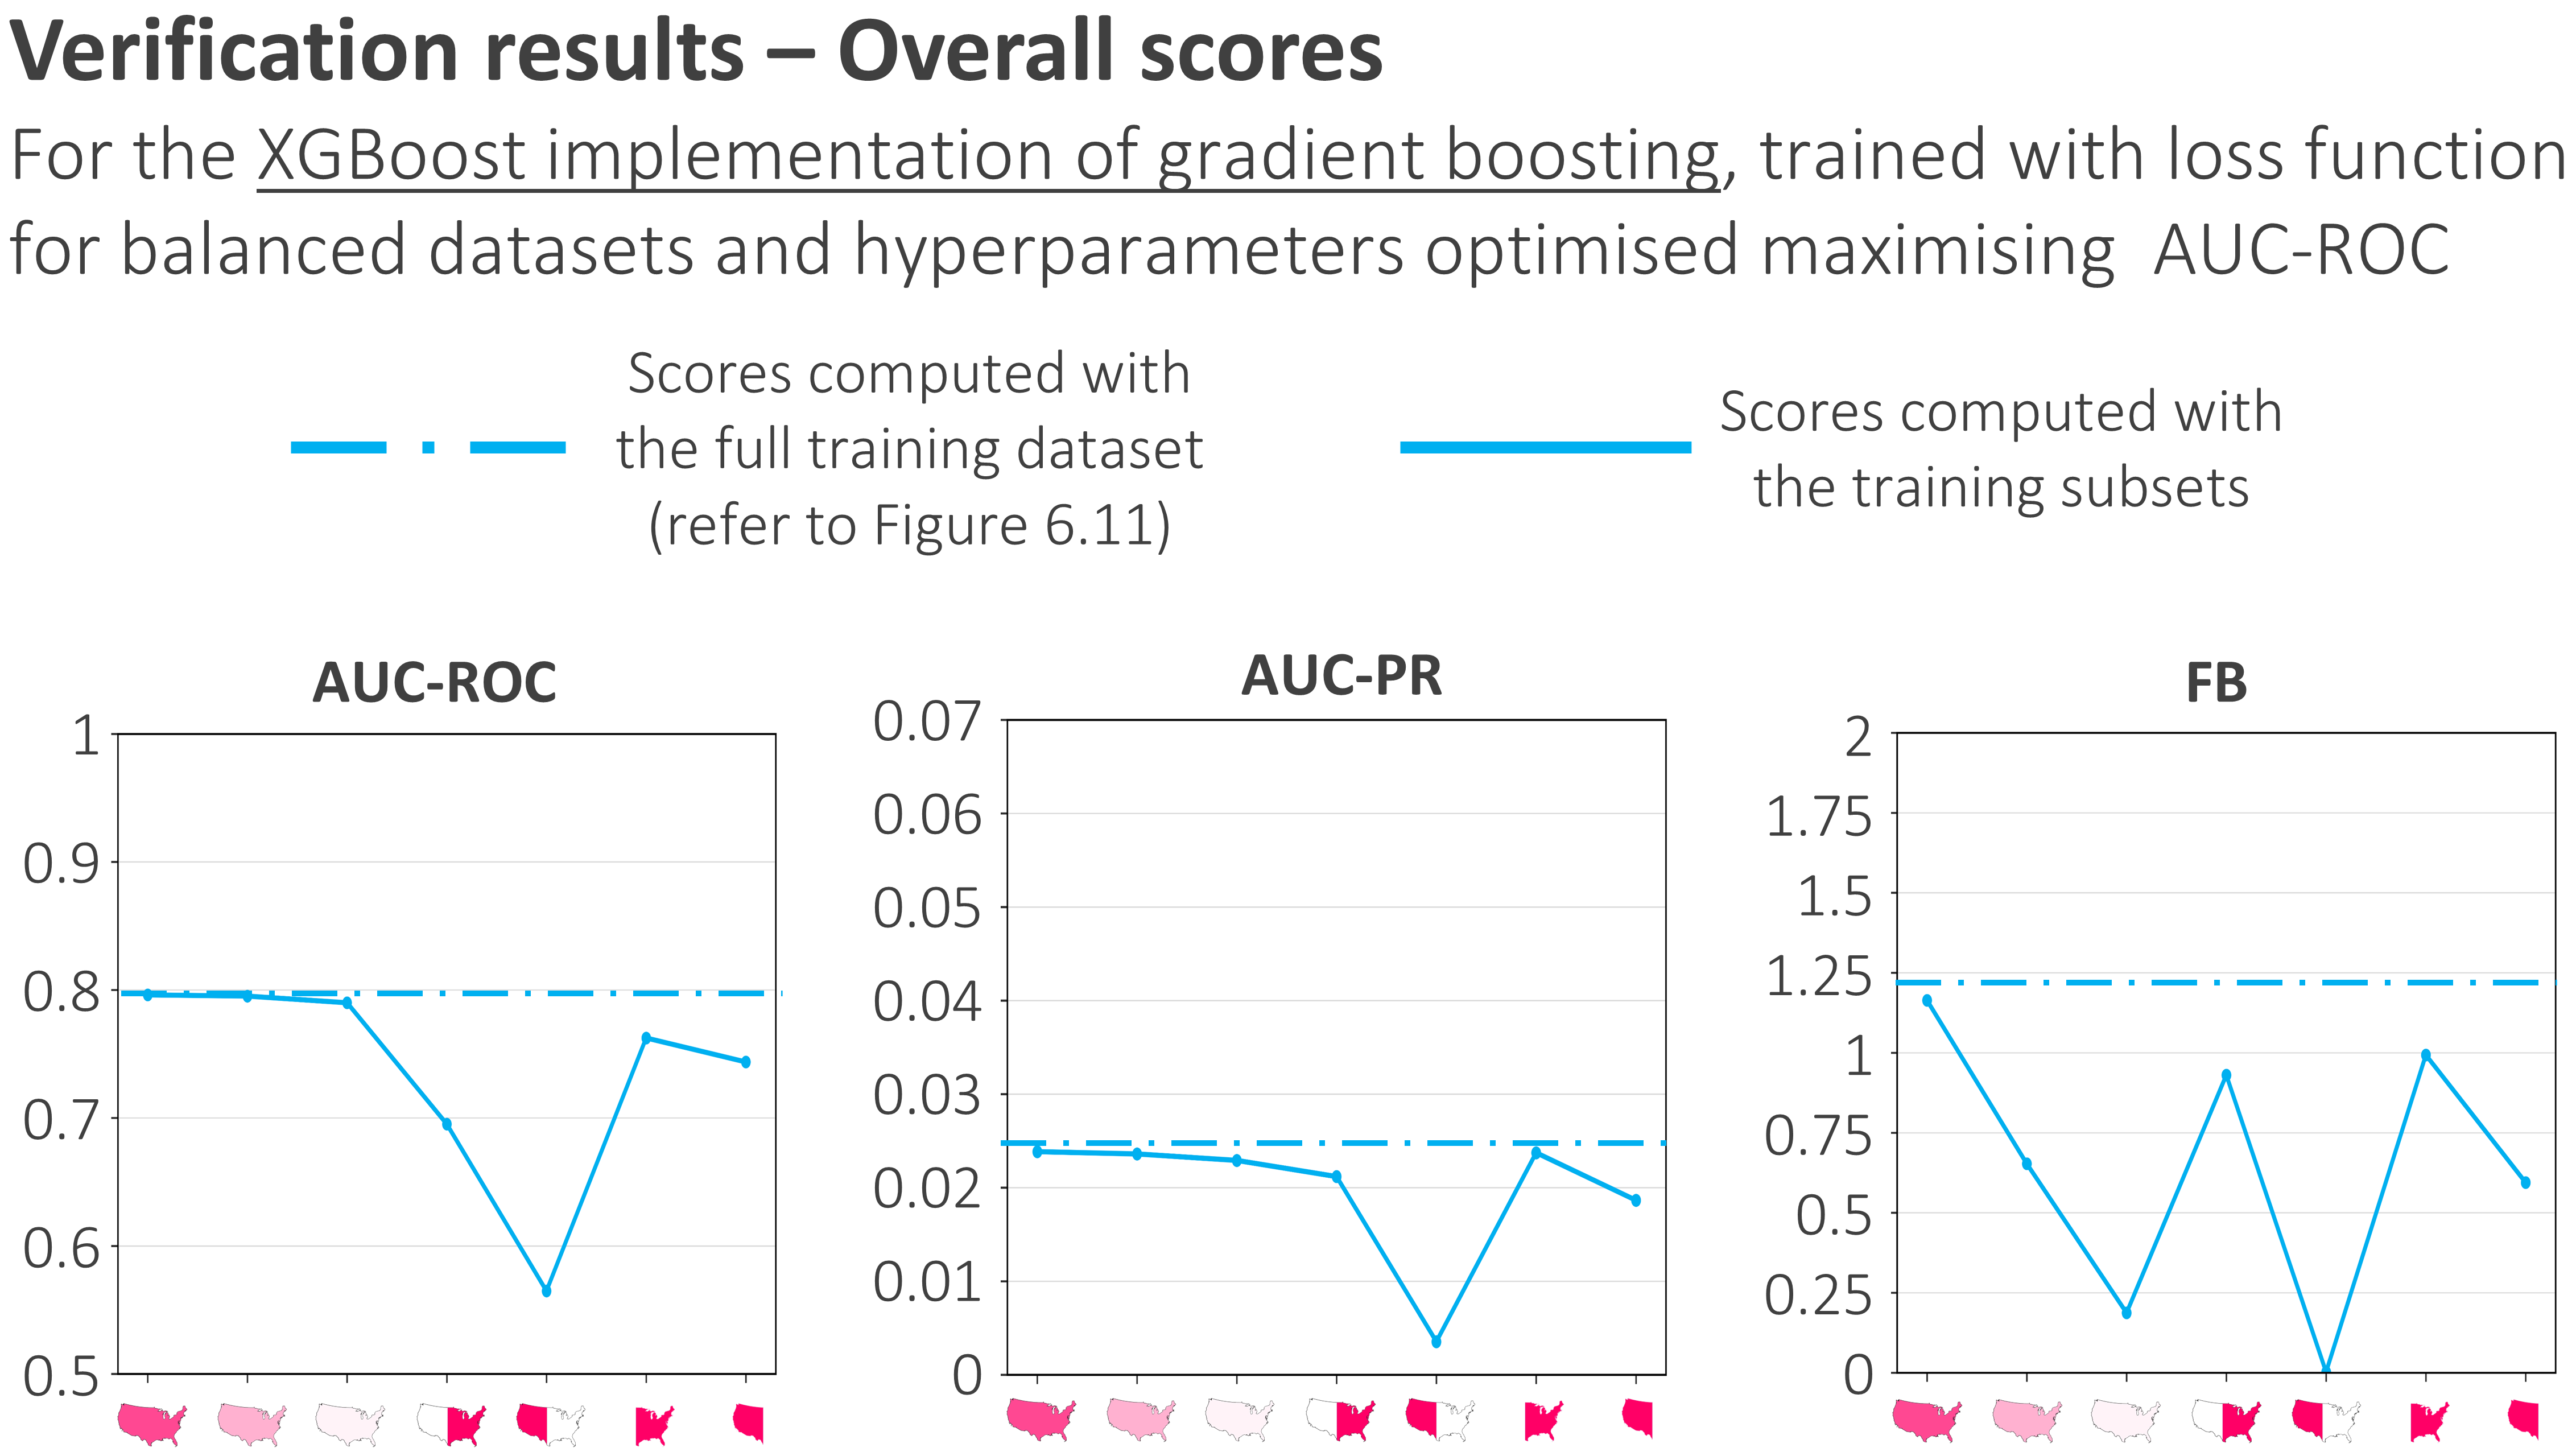
\includegraphics[width=\textwidth]{verif_overall_scores.png}
\caption{\textbf{Objective verification: overall scores (AUC-ROC, AUC-PR, FB)} Panel (a) shows the area under the ROC curve (AUC-ROC), computed for the XGBoost implementation of gradient boosting, trained with the loss function for balanced datasets and hyperparameters optimised to maximise AUC-ROC (as developed in Chapter \ref{data_driven_flash_floods_short_medium_range}). The score is computed with data from the \textcolor{colourTest}{verification} dataset (from 2021 to 2024). The solid line shows the scores computed using the three considered training approaches (TA1-3) as described in Figure \ref{fig:training_approaches}. The dashed line represents the score obtained when the model was trained with the full training dataset (refer to Figure \ref{fig:verif_training_test_overall}a. Panels (b) and (c) show, respectively, the area under the precision-recall curve and the frequency bias. Refer to Figures \ref{fig:verif_training_test_overall}e and \ref{fig:verif_training_test_overall}i for the corresponding scores obtained when the model was trained with the full training dataset.}
\label{fig:verif_overall_scores}
\end{figure}

When \marginpara{Objective verification: breakdown scores (ROC curves)} considering the ROC curves for TA1, those computed with probability thresholds discretised every 0.01\% (dashed lines in Figures \ref{fig: verif_breakdown_scores_roc_curve}b-c) show negligible difference in shape to that computed with the full training dataset (dashed line in Figure \ref{fig: verif_breakdown_scores_roc_curve}a). However, when considering the ROC curves built with probability thresholds discretised every 1\% (solid lines in Figures \ref{fig: verif_breakdown_scores_roc_curve}b-d), the ROC curves get "squashed" towards the bottom-left corner of the unit square. Consequently, the values of AUC-ROC reduce from 0.652 for TA1-1 to values close to the "no-skill" threshold (equal to 0.5) for TA1-2 (0.588) and TA1-3 (0.512). As seen in Figure \ref{fig:verif_overall_scores}a, the training datasets in TA2 and TA3 show opposite discrimination abilities. TA2-1 (Figure \ref{fig: verif_breakdown_scores_roc_curve}e) and TA3-1 (Figure \ref{fig: verif_breakdown_scores_roc_curve}g), with flash flood reports in the West part of the CONUS, show the poorest ROC curves. In particular, the ROC curve for TA2-1 shows that the model trained with this dataset has no discrimination ability. In contrast, the models trained with the TA2-2 (Figure \ref{fig: verif_breakdown_scores_roc_curve}f) and TA3-2 (Figure \ref{fig: verif_breakdown_scores_roc_curve}h) datasets show the closest ROC curves (with both discretisations) to the one trained with the complete training dataset (Figure \ref{fig: verif_breakdown_scores_roc_curve}a). The only difference lies in the shape of the dashed ROC curves for TA2-2 and TA3-2. For very small probabilities of exceedance (< 0.1\%), the ROC curves are squashed to the diagonal of the unit square, showing that the model has no discriminative ability when forecasts produce very small probabilities of exceedance. 

\begin{figure}[htbp]
\centering
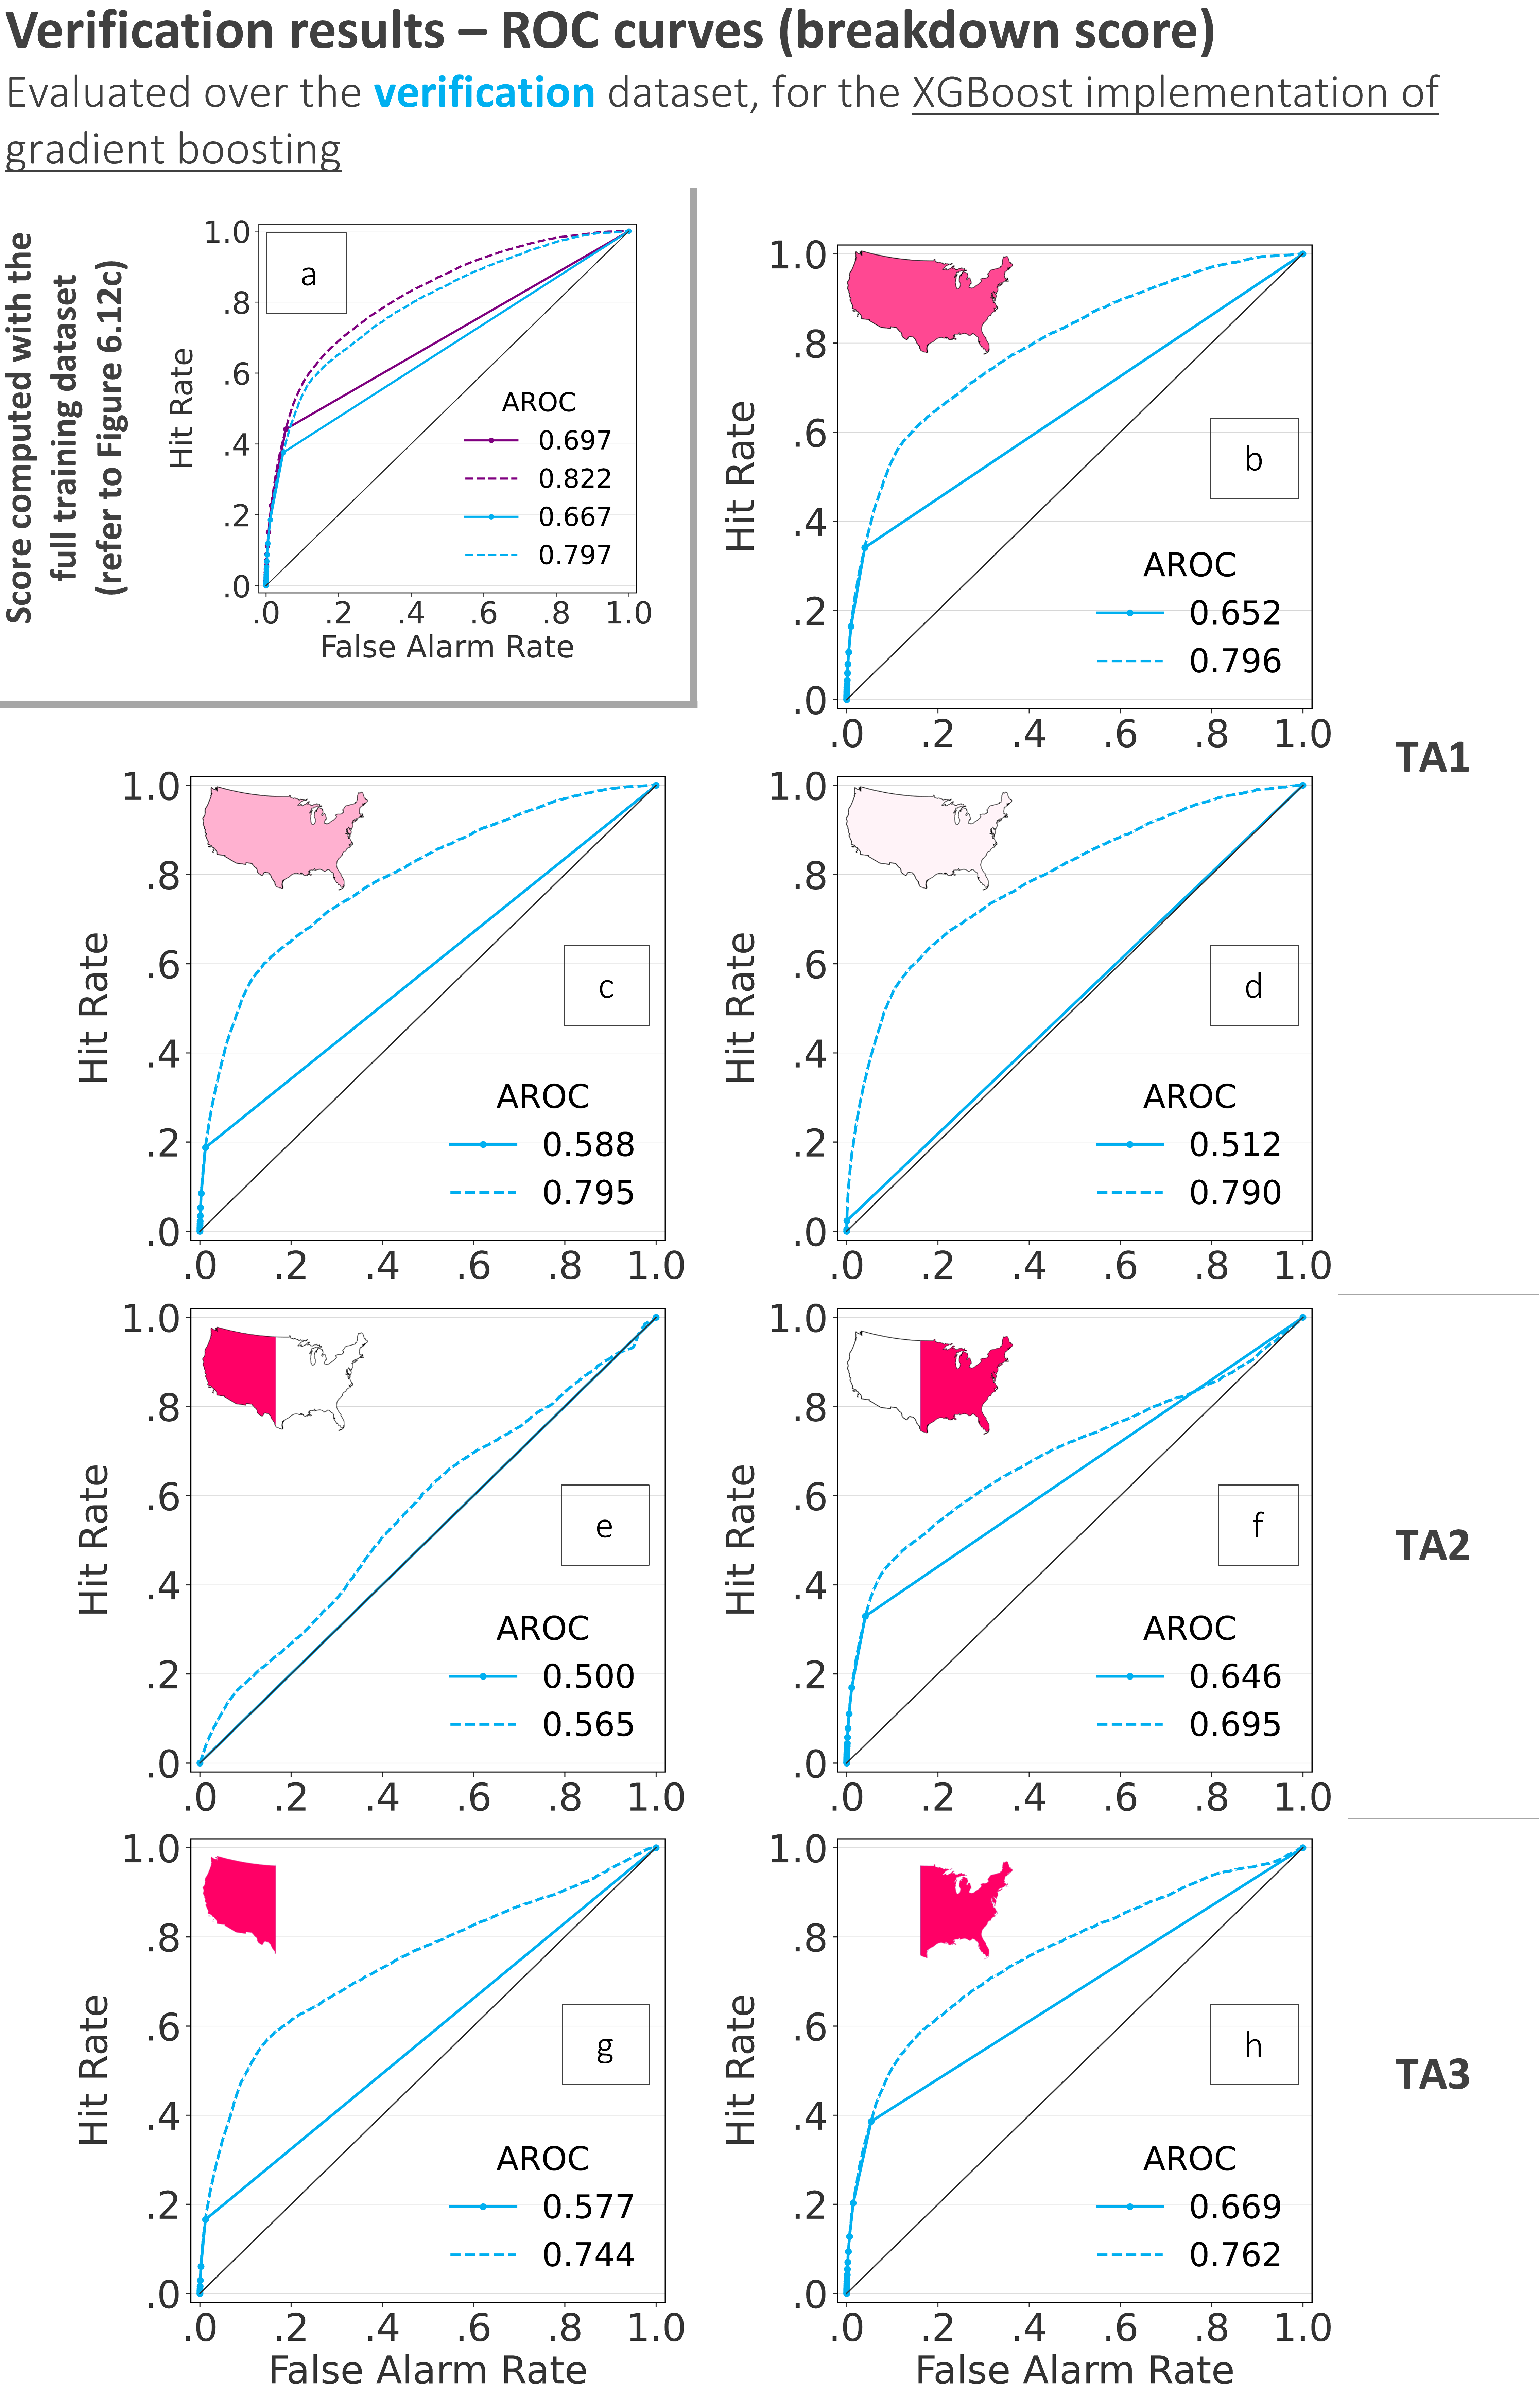
\includegraphics[scale = 0.95]{verif_breakdown_scores_roc_curve.png}
\caption{\textbf{Objective verification: breakdown scores (ROC curves)} ROC curves are shown for the XGBoost implementation of gradient boosting, trained with the loss function for balanced datasets and hyperparameters optimised to maximise AUC-ROC (developed in Chapter \ref{data_driven_flash_floods_short_medium_range}). Panel (a) shows the ROC curve for the model trained with the full trained dataset (as shown also in Figure \ref{fig:verif_training_test_breakdown_roc_curve}c, for the \textcolor{colourTraining}{training} dataset (from 2001 to 2020) and the \textcolor{colourTest}{verification} dataset (from 2021 to 2024)). Panels (b) to (d) show the ROC curves for the model trained with the training subset corresponding to training approach 1 (TA1), only for the \textcolor{colourTest}{verification} dataset. Panels (e) and (f) show the ROC curves obtained for TA2, while panels (g) and (h) show the ROC curves obtained for TA3. The ROC curves drawn with solid lines correspond to a probability discretisation of 1\%, with probabilities of exceedance ranging from 0 to 99\%. The ROC curves drawn with dashed lines correspond to a probability discretisation of 0.01\%, with probabilities of exceedance ranging up to values that depend on the TA, and shown in Figure \ref{fig:training_approaches}.}
\label{fig:verif_breakdown_scores_roc_curve}
\end{figure}

All \marginpara{Objective verification: breakdown scores (precision-recall curves)} the precision-recall curves have a similar shape to that obtained by the model trained with the full training dataset (Figure \ref{fig: verif_breakdown_scores_roc_curve}a). For TA1 (Figure \ref{fig: verif_breakdown_scores_roc_curve}b-c), the precision at very small values of recall increases with increasing reductions of flash flood reports in the training datasets. In contrast, the values of recall produced by the models decrease. Again, TA2-1 (Figure \ref{fig: verif_breakdown_scores_roc_curve}e) and TA3-1 (Figure \ref{fig: verif_breakdown_scores_roc_curve}g) correspond to the training approaches showing the worst performance. Both are capable of producing only very small values of recall, and TA2-1 also produces values of precision that are extremely low and close to 0. In contrast, TA2-2 (Figure \ref{fig: verif_breakdown_scores_roc_curve}f) and TA3-2 (Figure \ref{fig: verif_breakdown_scores_roc_curve}h) show the best precision-recall curves, achieving both high values of precision and recall. 

\begin{figure}[htbp]
\centering
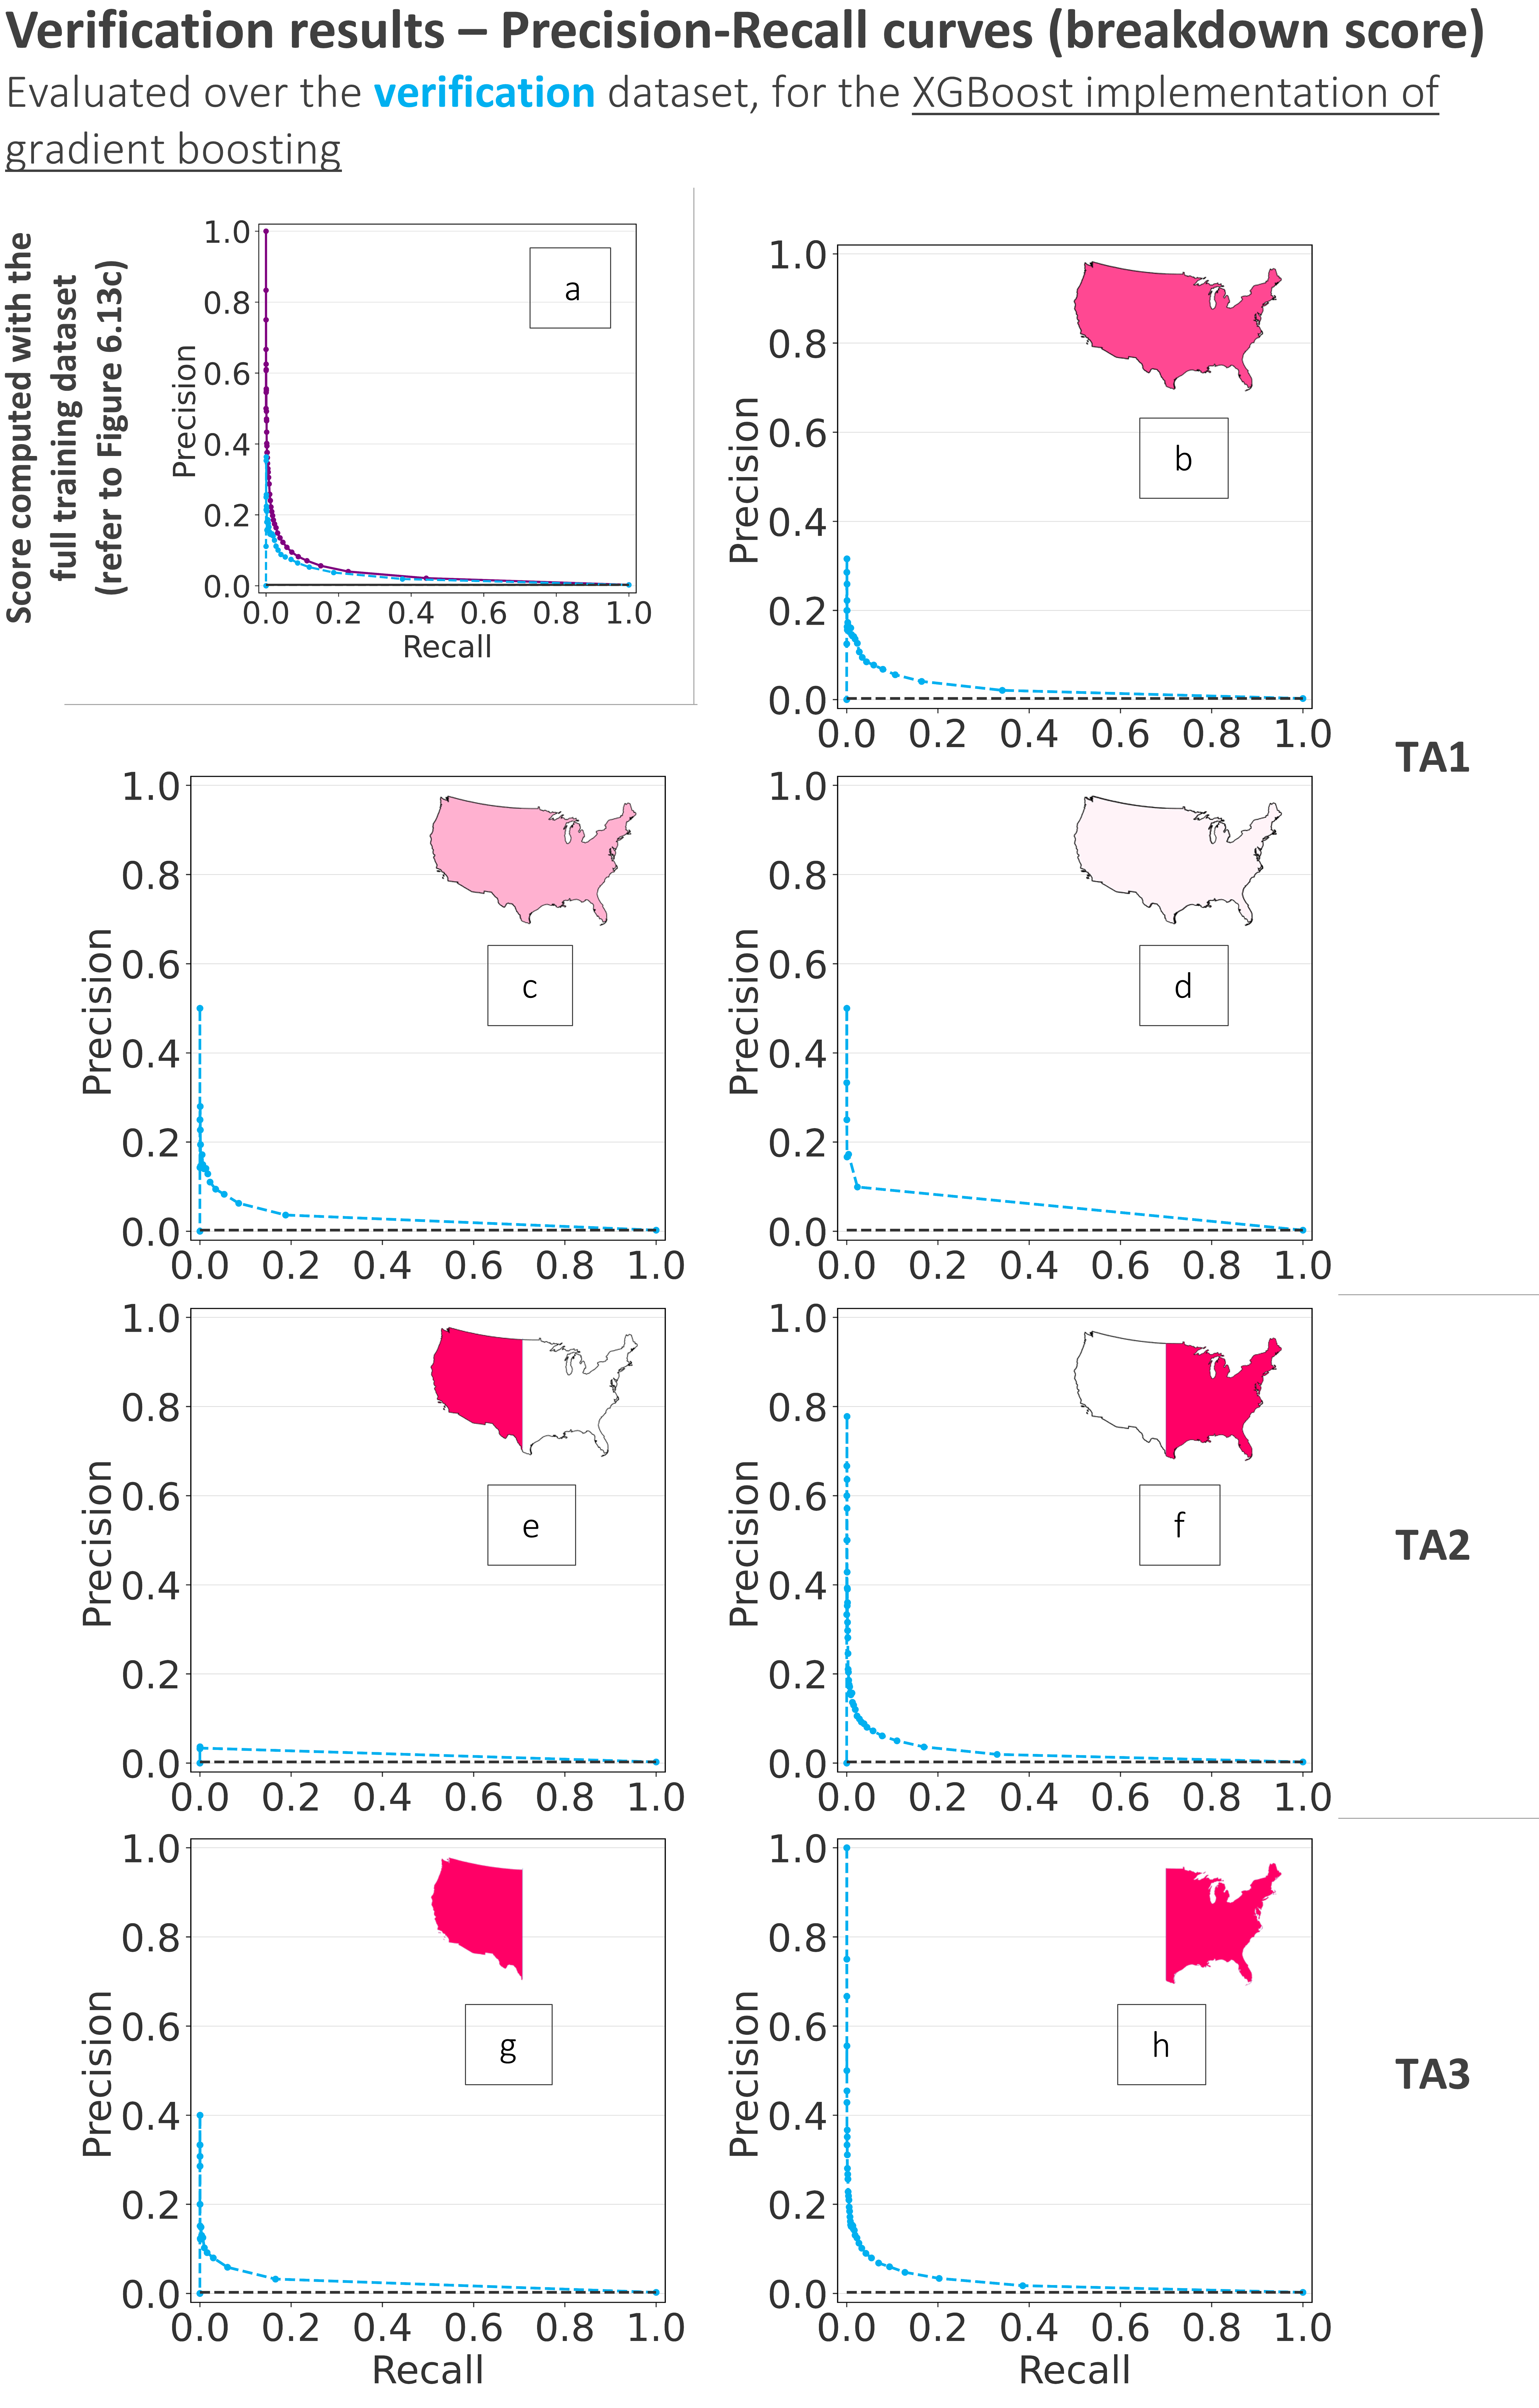
\includegraphics[scale = 0.95]{verif_breakdown_scores_pr_curve.png}
\caption{\textbf{Objective verification: breakdown scores (Precision-Recall curves)} Precision-Recall curves are shown for the XGBoost implementation of gradient boosting, trained with the loss function for balanced datasets and hyperparameters optimised to maximise AUC-ROC (developed in Chapter \ref{data_driven_flash_floods_short_medium_range}). Panel (a) shows the precision-recall curve for the model trained with the full trained dataset (as shown also in Figure \ref{fig:verif_training_test_breakdown_pr_curve}c, for the \textcolor{colourTraining}{training} dataset (from 2001 to 2020) and the \textcolor{colourTest}{verification} dataset (from 2021 to 2024)). Panels (b) to (d) show the precision-recall curves for the model trained with the training subset corresponding to training approach 1 (TA1), only for the \textcolor{colourTest}{verification} dataset. Panels (e) and (f) show the ROC curves obtained for TA2, while panels (g) and (h) show the ROC curves obtained for TA3. The ROC curves drawn with solid lines correspond to a probability discretisation of 1\%, with probabilities of exceedance ranging from 0 to 99\%. The ROC curves drawn with dashed lines correspond to a probability discretisation of 0.01\%, with probabilities of exceedance ranging up to values that depend on the TA, and shown in Figure \ref{fig:training_approaches}.}
\label{fig:verif_breakdown_scores_pr_curve}
\end{figure}

The \marginpara{Objective verification: breakdown scores (reliability diagrams)} reliability diagrams for TA1-1 Figure \ref{fig: verif_breakdown_scores_reliability_diagram}b, TA2-2 Figure \ref{fig: verif_breakdown_scores_reliability_diagram}f, and TA3-2 Figure \ref{fig: verif_breakdown_scores_reliability_diagram}h show very similar reliability to that obtained by the model trained with the complete training dataset (Figure \ref{fig: verif_breakdown_scores_reliability_diagram}a): forecast probabilities below \sim20\% remain fairly reliable (as they overlap with the diagonal), and the probabilities produced by the model remain between 30 and 40\%. The forecast probabilities for TA1-2 (Figure \ref{fig: verif_breakdown_scores_reliability_diagram}c) remain overall reliable, but the model is not able to produce probabilities bigger than \sim20\%. When considering TA1-3 (Figure \ref{fig: verif_breakdown_scores_reliability_diagram}d), the model is producing very small forecast probabilities that, overall, underestimate the observed frequency of flash floods (the diagram lies above the diagonal). The model trained with TA3-1 (Figure \ref{fig: verif_breakdown_scores_reliability_diagram}g) shows a similar behaviour to TA1-3. Finally, TA2-1 (Figure \ref{fig: verif_breakdown_scores_reliability_diagram}e) shows an almost inexistent reliability diagram, showing that the model is producing very small probabilities of flash flood occurrence.   

\begin{figure}[htbp]
\centering
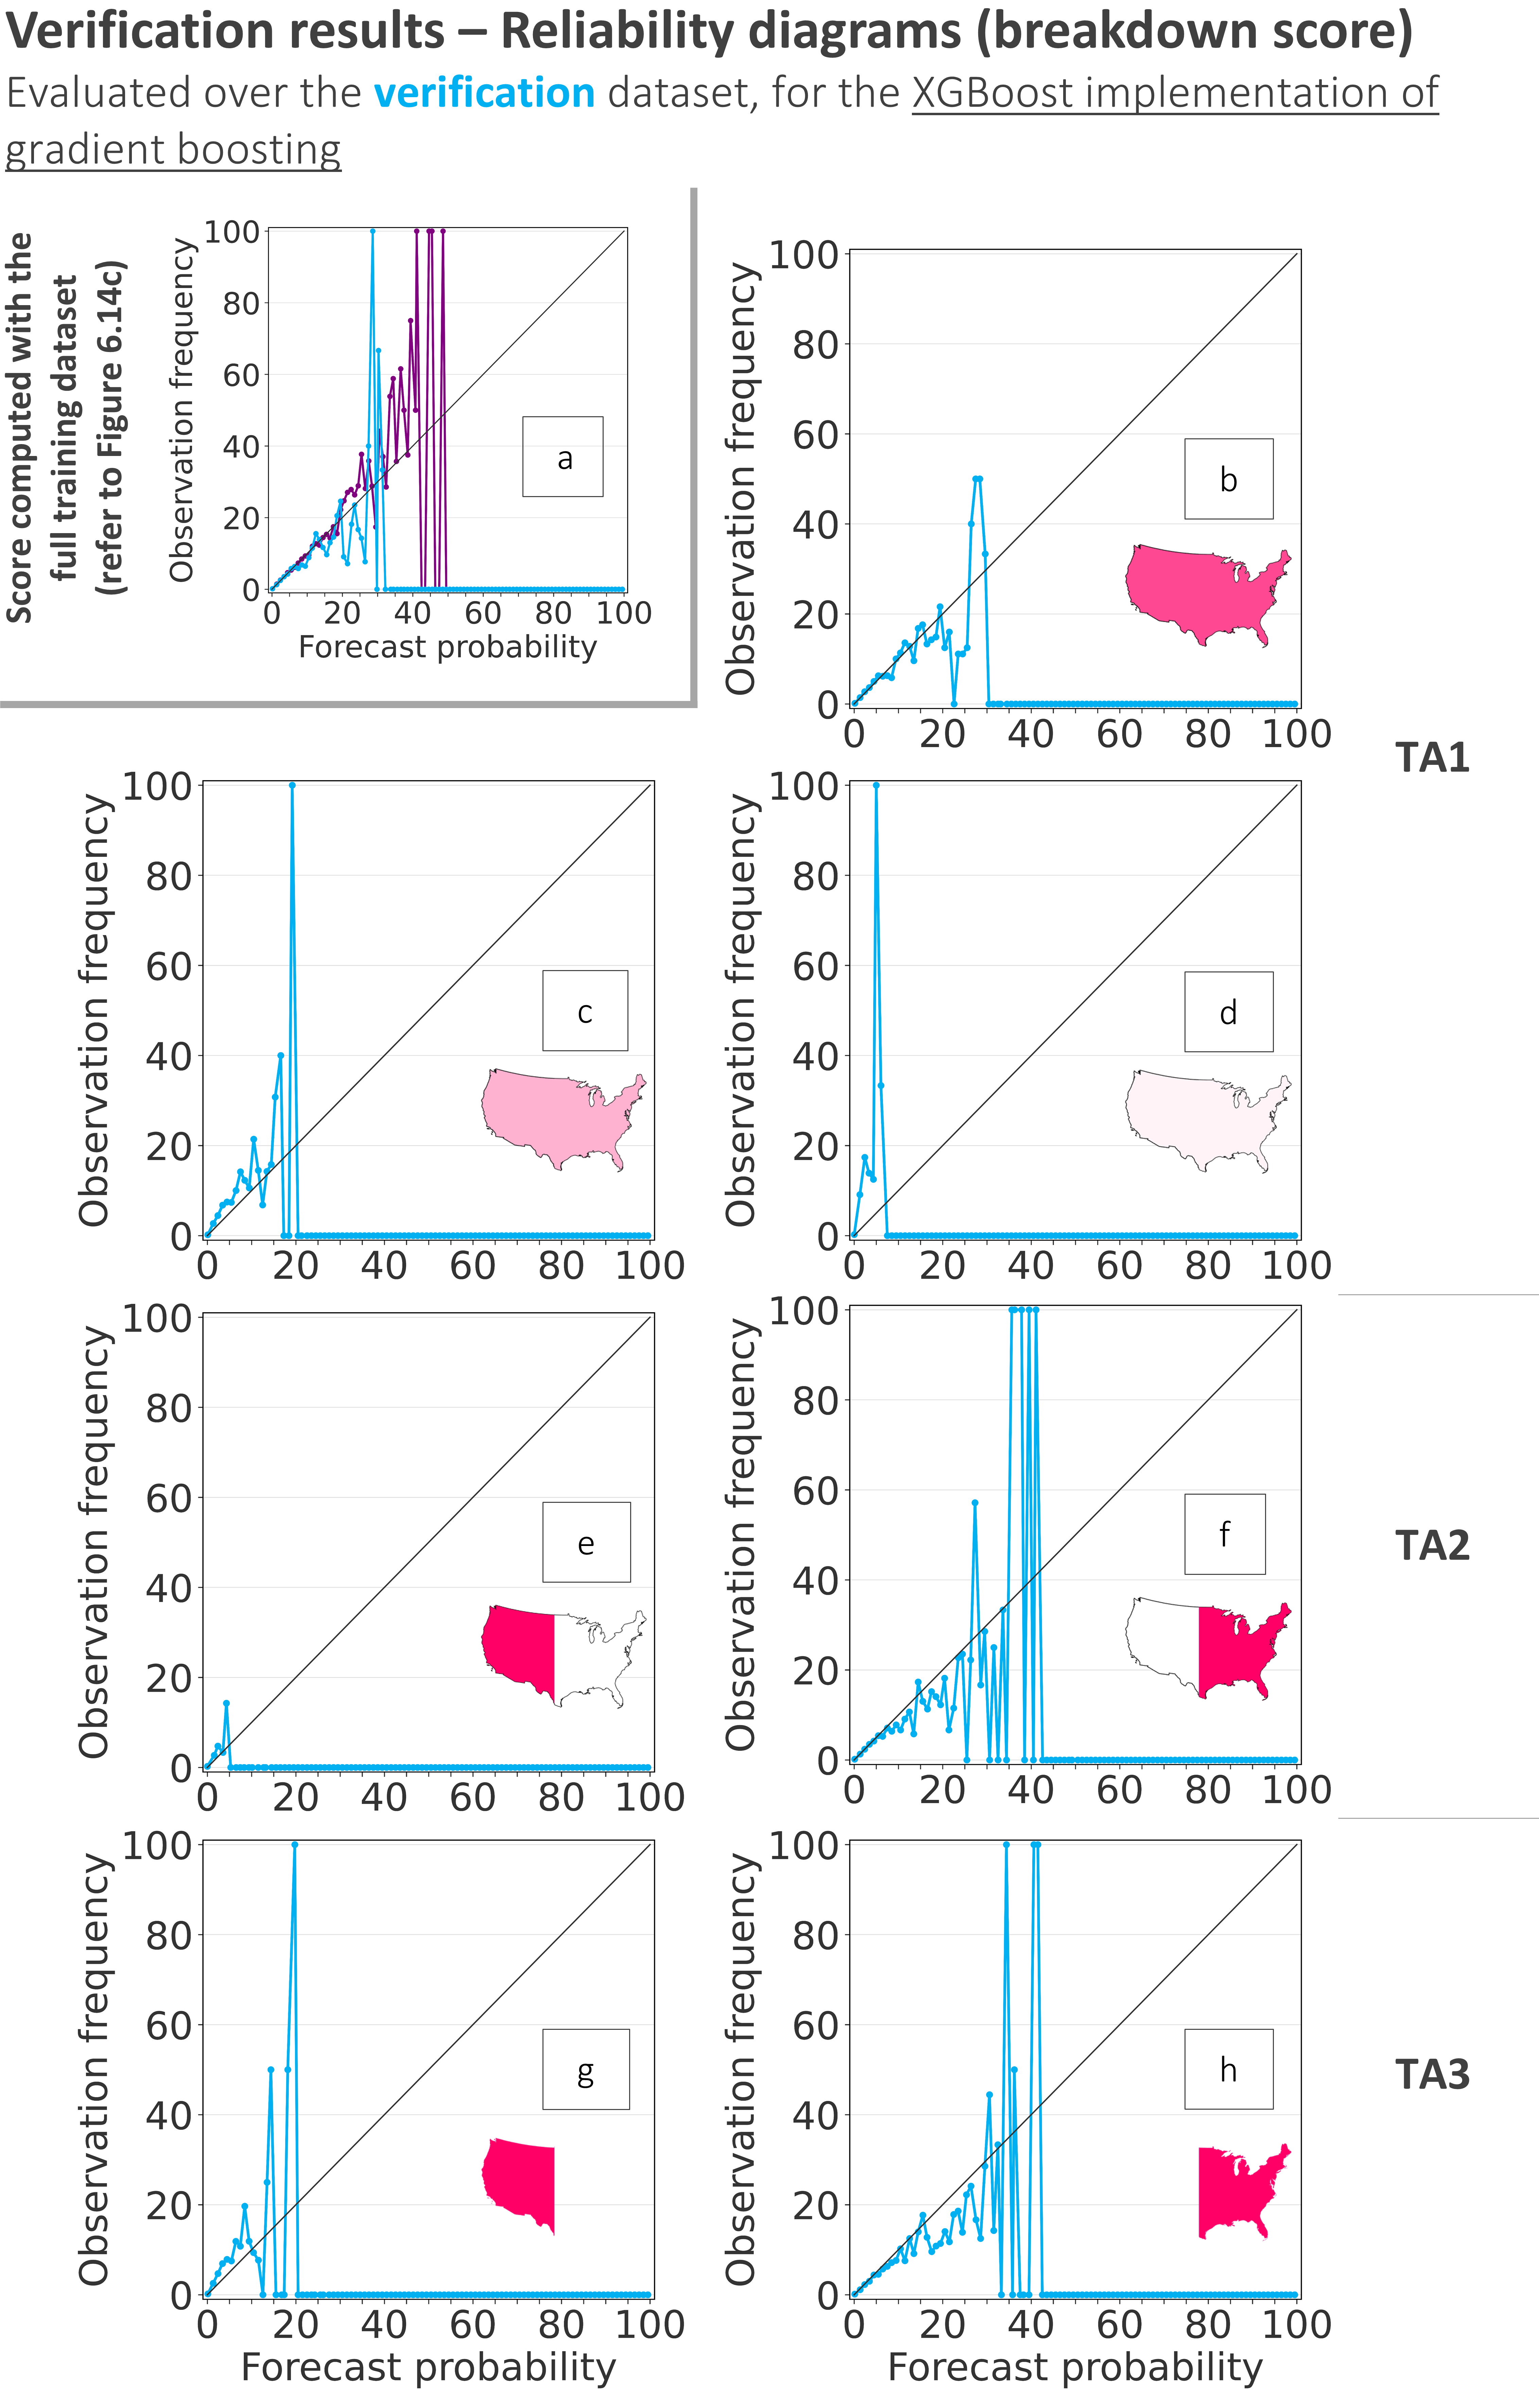
\includegraphics[scale = 0.95]{verif_breakdown_scores_reliability_diagram.png}
\caption{\textbf{Objective verification: breakdown scores (Reliability Diagrams)} Precision-Recall curves are shown for the XGBoost implementation of gradient boosting, trained with the loss function for balanced datasets and hyperparameters optimised to maximise AUC-ROC (developed in Chapter \ref{data_driven_flash_floods_short_medium_range}). Panel (a) shows the precision-recall curve for the model trained with the full trained dataset (as shown also in Figure \ref{fig:verif_training_test_breakdown_reliability_diagram}c, for the \textcolor{colourTraining}{training} dataset (from 2001 to 2020) and the \textcolor{colourTest}{verification} dataset (from 2021 to 2024)). Panels (b) to (d) show the precision-recall curves for the model trained with the training subset corresponding to training approach 1 (TA1), only for the \textcolor{colourTest}{verification} dataset. Panels (e) and (f) show the ROC curves obtained for TA2, while panels (g) and (h) show the ROC curves obtained for TA3. The ROC curves drawn with solid lines correspond to a probability discretisation of 1\%, with probabilities of exceedance ranging from 0 to 99\%. The ROC curves drawn with dashed lines correspond to a probability discretisation of 0.01\%, with probabilities of exceedance ranging up to values that depend on the TA, and shown in Figure \ref{fig:training_approaches}.}
\label{fig:verif_breakdown_scores_reliability_diagram}
\end{figure}


%%%%%%%%%%%%%%%%%%%%%
\section{Discussions}
\label{regional_to_global_training_discussions}

Amongst \marginpara{TA3 emerges as the most promising approach for developing predictions of areas at risk of flash floods from geographically-limited training data, especially when carefully selecting training regions that maximise hydro-climatological diversity and observational density.} all evaluated strategies, TA3 emerges as the most promising approach for developing predictions of areas at risk of flash floods from geographically-limited training data. Models exposed exclusively to data-rich regions during training have been shown here to extrapolate forecast probabilities in ungauged areas that resemble those as if the model had been trained with data over the whole domain. This shows that the specific data-driven model used in this chapter (XGBoost implementation for gradient boosting) can learn general flash-flood-triggering hydro-meteorological patterns and preserve the integrity of the learned probability distributions, enabling reliable predictions when encountering similar hydro-meteorological conditions in previously unseen geographical domains. This finding aligns with evidence presented in \citet{Kratzert_2024}, who demonstrated similar transferability of learned hydro-meteorological relationships for riverine flood prediction, suggesting that data-driven approaches can capture fundamental hydrological processes that transcend specific geographical boundaries. However, not all regions with observations may perform equally. The higher performance of TA3-2 (training dataset over the \textit{east} side of the CONUS) over TA3-1 (training dataset over the \textit{west} side) demonstrates the critical importance of selecting regions that maximise hydro-climatological diversity and observational density. By utilising the eastern CONUS — a region characterised by diverse precipitation regimes, varied topography, and relatively high flash flood frequency — the model learned generalisable patterns that were successfully transferred to predict areas at risk of flash floods in unseen regions (in this case, the Western side of the CONUS). 

TA1 \marginpara{The alternative training approaches (TA1 and TA2) reveal fundamental limitations that render them unsuitable for the global extension of regionally-trained models.} showed that full-domain but sparse coverage produces models with progressively degraded performance (both in reliability and discrimination ability) as the observational density decreases. The data-driven model became severely underperforming with large reductions in observational density (90\% in TA1-3). In this case, the data-driven model trained with such a severe lack of observations cannot learn general hydro-meteorological patterns that may trigger flash floods. This is exemplified by the ROC curve built with operationally-relevant probability thresholds (not lower than 1\%) that mostly overlap with the diagonal, which is typical of a model with no discrimination ability. The model's reliability is also very poor, showing a systematic shift towards severe under-prediction seen in the reliability diagram and in the frequency bias. The model's systematic failure in predicting areas at risk of flash floods appears even more evident by examining the precision-recall curves. When the curve displays only a short segment before terminating at low recall values, this indicates that the model has learned to make positive predictions for only a minuscule fraction of the evaluation data, essentially defaulting to negative predictions beyond a very conservative probability threshold. This behaviour also manifests a paradoxical relationship between training data availability and initial precision: models trained with fewer positive reports often achieve higher precision at very low recall values compared to those trained on more comprehensive datasets. This counterintuitive result arises because extreme data scarcity forces data-driven models to become hyper-conservative, triggering positive predictions only under conditions that almost exactly match their limited training examples. Whilst this extreme selectivity yields high precision for the few predictions made, it comes at the cost of missing the vast majority of actual positive cases. In contrast, models trained with more diverse positive examples learn richer representations that enable generalisation across varied flash flood contexts. Although this broader learning results in lower precision at the beginning of the precision-recall curve because the model attempts to capture a wider range of conditions (also at the cost of including more false alarms), these models ultimately provide operationally viable performance by maintaining reasonable precision across meaningful recall levels. For flash flood prediction systems, where the failure to detect events has potentially fatal consequences, the ability to identify hazards across their full diversity of occurrence patterns far outweighs the superficial advantage of perfect precision limited to an insignificant fraction of events, underscoring the critical importance of guaranteeing exposure to sufficient flash flood occurrences to the model. Similar results, therefore, would be obtained if we were to train a data-driven model with global impact reports from databases such as EM-DAT. TA2 shows contrasting performances. TA2-2, despite being exposed during training to western regions appearing to have zero flash flood occurrences, successfully generalises learned patterns to these ostensibly flood-free areas, achieving performance metrics approaching those of the baseline model. This success stems from the eastern CONUS encompassing diverse hydro-climatic regions — from humid subtropical to continental climates — and experiencing relatively high flash flood frequency, providing sufficiently rich training signals to capture the fundamental relationships between atmospheric forcing, land surface characteristics, and flash flood occurrence. The model's ability to extrapolate these learned patterns to the semi-arid western regions, despite never observing positive examples there during training, suggests that the diversity and density of eastern observations can compensate for the artificial absence of western reports. Crucially, this compensatory capability proves highly sensitive to training data quality: when the same approach is applied using western data (TA2-1), the limited hydro-climatic diversity and lower flash flood frequency in the Western side of the CONUS fail to provide adequate training signals, resulting in an extremely poor performance over the unseen areas.

The \marginpara{Objectively verifying the global data-driven predictions remains challenging due to the lack of observations} absence of comprehensive global impact observations prevents rigorous global objective verification of the forecasts. Global disaster databases such as EM-DAT and DesInventar, though invaluable for large-scale impact assessment, exhibit severe reporting biases, typically capturing only events exceeding mortality or economic thresholds and systematically under-representing more minor flash floods that can also cause substantial local impacts. There also exist spatial biases, with reporting quality correlating strongly with institutional capacity, media coverage, and proximity to urban centres, precisely inverse to the distribution of vulnerability. This verification gap forces reliance on case study analyses, as demonstrated in this research, which, whilst providing valuable insights into model behaviour for specific high-impact events, cannot establish robust statistics about forecast performance critical to bridge the gap between methodological capability and operational confidence. Meteorological services must issue warnings based on models whose performance remains statistically unquantified in their regions, whilst international donors and governments must allocate resources to prediction systems whose local accuracy cannot be systematically demonstrated. Future solutions may emerge through adopting less standard observations to bulk current databases or create ones that take into account more minor local events but potentially equally impactful as those already included in the most commonly used impact databases. Satellite-detected flooding could be leveraged as a proxy for ground impacts. Crowdsourced observations from citizen scientists and social media streams could offer real-time flood impact information that could validate and calibrate predictions, yet extracting reliable information from noisy, biased social data requires advanced natural language processing and verification protocols. The integration of Internet of Things (IoT) devices, including low-cost weather stations and water level sensors, promises to dramatically expand observational coverage, though sustainability concerns regarding maintenance, calibration, and data transmission in resource-limited settings must be addressed. 

Whilst \marginpara{Operational deployment may also be a challenge} this research establishes the methodological foundation for global prediction of areas at risk of flash flood, the transition from research demonstration to operational deployment presents challenges that merit careful consideration. Training a model operating at the spatial resolutions preferred in flash flood prediction (typically under 10 km) across global domains would require substantial computational resources, particularly if ensemble forecasts are developed to quantify uncertainty. Whilst at inference time, data-driven model are extremely cheap to run (even at high resolutions), training such a model might require considerable technological resources available only in a handful of centres such as ECMWF which already develops GloFAS. Model updating strategies present another layer of complexity—the continuous integration of new flash flood observations could improve prediction accuracy, but requires automated quality control procedures and regular retraining cycles that demand both computational resources and human oversight. 

The \marginpara{Extension to multi-hazard early warning frameworks} transfer learning framework demonstrated in this chapter for flash floods addresses a fundamental challenge shared across numerous hydro-meteorological hazards, i.e., the existence of high-quality regional datasets alongside the absence of comprehensive global observations. Lightning strikes, for instance, benefit from dense ground-based detection networks in North America (National Lightning Detection Network\footnote{https://www.vaisala.com/en/products/national-lightning-detection-network-nldn}) and Europe (EUCLID\footnote{https://www.euclid.org/}), yet vast regions across Africa, Asia, and South America remain unmonitored despite experiencing intense thunderstorm activity. Similarly, landslide inventories such as the USGS Landslide Inventory\footnote{https://www.usgs.gov/tools/us-landslide-inventory-and-susceptibility-map} in the US or the Italian IFFI database\footnote{https://www.progettoiffi.isprambiente.it/?lang=en} offer detailed historical records within specific regions, whilst global databases remain sparse and inconsistent. The methodological framework established here — training models on hydro-meteorologically diverse regions with quality observations, and then applying them globally — could be directly adapted to other hazards such as those just mentioned. For lightning prediction, models trained on the North American or European observational datasets could learn relationships between atmospheric conditions and lightning occurrence, subsequently providing life-saving predictions in regions where agricultural workers and school children face significant lightning mortality without warning systems. Landslide susceptibility models developed using comprehensive inventories from mountainous regions in Europe or Japan could be transferred to predict this hazard in data-scarce mountainous areas across the Andes or Himalayas.

The \marginpara{Climate change adaptation and model robustness under non-stationarity} demonstrated transferability of flash flood predictions across diverse hydro-climatic regions carries profound implications for climate change adaptation strategies. As global warming intensifies the hydrological cycle, regions historically experiencing infrequent flash flooding may transition into high-risk zones, whilst traditional flood-prone areas may face unprecedented extremes. The success of models trained on the climatologically diverse eastern CONUS in predicting flash floods in semi-arid western regions suggests that current data-driven approaches could provide anticipatory warning capabilities for communities entering unfamiliar climate regimes. However, this raises critical questions about model robustness under non-stationary conditions: how frequently must models be retrained to capture evolving precipitation-runoff relationships, and can transfer learning approaches trained on present-day extreme events adequately predict future extremes that may exceed historical analogues? The answer to these questions is tentatively positive, because even though specific verification for flash flood occurrence is needed, positive signals in this direction have already been presented in the literature \citep{Bertola_2023}. Moreover, through the development of a historical dataset of flash flood occurrence by running the data-driven model on retrospective reanalysis data, it would be possible to create climatological studies to assess increased/decreased frequency of flash floods in a particular region, or better understand the hydro-meteorological patterns that generate flash flood occurrence. 


%%%%%%%%%%%%%%%%%%%%%
\section{Conclusions}
\label{regional_to_global_training_conclusions}

This chapter has systematically investigated the critical trade-offs between spatial coverage and observational density in developing transferable flash flood prediction models, addressing Research Question 3 of this thesis. Through comprehensive sensitivity analysis across three distinct training approaches, we have demonstrated that the aspiration to achieve global flash flood prediction coverage is methodologically feasible despite the severe paucity of observations in most regions worldwide.

The empirical evidence establishes that training over a domain with good observational data emerges (TA3) as the optimal strategy for extending regional models to global applications. This approach, whereby models train exclusively on data-rich regions before deployment to unseen areas, successfully preserves the integrity of learned hydro-meteorological relationships. The striking performance disparity between eastern-trained and western-trained models underscores, however, a fundamental principle: successful transfer learning requires training regions that encompass large enough hydro-climatological diversity and fairly high observation density. The eastern CONUS, with its varied precipitation regimes spanning humid subtropical to continental climates, provides the requisite diversity for models to learn generalisable flash flood generation mechanisms. Conversely, the systematic failures of alternative approaches illuminate critical constraints on global model development. Random spatial sampling (TA1) demonstrates that maintaining geographical coverage whilst reducing observation density produces catastrophic performance degradation, with models becoming hyper-conservative and operationally ineffective when positive examples become too sparse. The regionally-constrained training with global visibility (TA2) reveals an even more fundamental limitation: exposing models to regions with artificially absent flash flood observations may also severely corrupt the learning process.

Significant challenges remain before operational implementation can bridge the gap between methodological capability and life-saving warnings. Fore example, the absence of comprehensive global verification data prevents rigorous assessment of model performance precisely where it matters most, i.e., in vulnerable, data-scarce regions. In this chapter, impact reports only from the CONUS were considered; however, it is foreseen that strategic aggregation of data from diverse, well-monitored regions (such as Western Europe or selected countries such as Japan, Ecuador, or Brazil) could further improve the predictions computed for this thesis. It is also anticipated that innovative solutions, such as the use of other non-standard observations (satellite-derived inundation maps, crowdsourcing observations, and social media posts), will be applied to bulk current observational datasets, enabling objective validation analysis of global predictions. Moreover, it is also envisioned that the knowledge developed in this chapter about applying regionally-trained data-driven models to global applications might be extended to also low-probability, high-impact hazards such as landslides and lightning. Finally, as climate change drives communities into unfamiliar hazard regimes, the ability to transfer knowledge from observed to unobserved regions becomes increasingly critical for adaptation and resilience.